\documentclass[handout]{ximera}
\input{../preamble.tex}
\author{Mary E. Pilgrim, and implemented in Ximera by Liam Coulter}


\title{Spring 2017 Exam 3}

\begin{document}
\begin{abstract}
  Here you can work on a practice exam 3. This exam was administered in Spring 2017.
\end{abstract}
\maketitle

\begin{center}
\Large{Math 160 Calculus for Physical Scientists I \\ Exam 3 - Version 1 \\ April 13, 2017, 5:00-6:50 pm}
\end{center}



%%MC%%
%%Problem 1%%
\begin{problem}
Suppose that $f(x) = -2x^2+cx+d$ has a local maximum at the point (2, 4). What must the values of $c$ and $d$ be to satisfy these conditions?
\begin{multipleChoice}
    \choice [correct]{$c=8$, $d=-4$}
    \choice {$c=8$, $d=4$}
    \choice {$c=2$, $d=4$}
    \choice {$c=2$, $d=-4$}
    \choice {$c=-8$, $d=4$}
    \choice {None of the above}
\end{multipleChoice}
\end{problem}


%%Problem 2%%
\begin{problem}
Given that $\displaystyle\int_{-3}^0 Y(x) \,dx=7$, what is the value of $\displaystyle\int_{-3}^0 x-Y(x) \,dx$?
\begin{multipleChoice}
	\choice {$\displaystyle-\frac{9}{2}$}
	\choice [correct]{$\displaystyle-\frac{23}{2}$}
	\choice {$\displaystyle\frac{23}{2}$}
	\choice {$\displaystyle\frac{5}{2}$}
	\choice {$\displaystyle-\frac{5}{2}$}
	\choice {None of the above.}
\end{multipleChoice}
\end{problem}


%%Problem 3%%
\begin{problem}
The graph of $f$ is given below. Which of the following estimates is most accurate for the value of $\displaystyle\int_0^6 f(x)\, dx$?

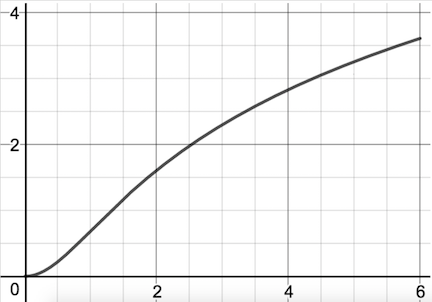
\includegraphics [scale=0.5]{Area-Ex3.png} %%This is a png version

\begin{multipleChoice}
	\choice {$6$}
	\choice [correct]{$12$}
	\choice {$18$}
	\choice {$24$}
\end{multipleChoice}
\end{problem}


%%Problem 4%%
\begin{problem}
Consider $Q(x)=\displaystyle\frac{1}{x^2+1}$

\begin{question}
What is the domain of $Q$?
\begin{multipleChoice}
	\choice {$(-\infty,-1)\cup(-1,1)\cup(1,\infty)$}
	\choice {$(-\infty,0)\cup(1,\infty)$}
	\choice [correct]{$(-\infty,\infty)$}
	\choice {$(-\infty,-1)\cup(-1,\infty)$}
\end{multipleChoice}
\end{question}

\begin{question}
What are the critical points of $Q$?
\begin{multipleChoice}
	\choice {$x=-1$, $x=1$}
	\choice [correct]{$x=0$}
	\choice {$x=-1$, $x=1$, $x=0$}
	\choice {$Q(x)$ does not have any critical points.}
\end{multipleChoice}
\end{question}

\end{problem}


%%Problem 5%%
\begin{problem}
The function $\displaystyle g(x) = \frac{1}{24}x^3+\sqrt{x}$ is concave down for all $x$ in the interval
\begin{multipleChoice}
	\choice [correct]{$(0,1)$}
	\choice {$(1,\infty)$}
	\choice {$(0,\infty)$}
	\choice {$g(x)$ is never concave down.}
\end{multipleChoice}
\end{problem}


%%Problem 6%%
\begin{problem}
What are the inflection points of $F(x)=x^4-4x^3+6x^2+1$?
\begin{multipleChoice}
	\choice {$x=0$}
	\choice {$x=1$}
	\choice [correct]{$F(x)$ does not have any inflection points.}
\end{multipleChoice}
\end{problem}


%%Problem 7%%
\begin{problem}
Suppose that $f'(x)$ is continuous and differentiable on its domain, $f'(B)=0$, and $f(x)$ has a local minimum at $x=B$. Then which of the following statements is true? Select all applicable answers.
\begin{selectAll}
	\choice [correct]{$f'(x)$ changes from negative to positive at $x=B$ (as $x$ increases).}
	\choice {$f'(x)$ changes from positive to negative at $x=B$ (as $x$ increases).}
	\choice {$f''(B)<0$.} 
	\choice [correct]{$f''(B)>0$.}
	\choice {$f''(B)=0$.}
	\choice {None of the above.}
\end{selectAll}
\end{problem}


%%Problem 8%%
\begin{problem}
Suppose that $R'(x)$ is differentiable, increasing, and negative on $[-1,1]$. Then $R(x)$


\begin{multipleChoice}
	\choice {is increasing and concave down on $(-1,1)$.}
	\choice {is decreasing and concave down on $(-1,1)$.}
	\choice [correct]{is increasing and concave up on $(-1,1)$.}
	\choice {is decreasing and concave up on $(-1,1)$.}
	\choice {has a local min at $x=0$.}
	\choice {None of the above.}
\end{multipleChoice}
\end{problem}


%%Problem 9%%
\begin{problem}
Suppose that $P''(t)=6t-1$. Given that $P(t)$ has a horizontal tangent at $t=-3$ and passes through the point $(-1,\frac{1}{2})$, what are $P'(t)$ and $P(t)$?
\begin{question}
	\[
	\displaystyle P'(t) =    \answer[given]{3t^{2}-t+30 }
	\]
\end{question}

\begin{question}
	\[
	\displaystyle P(t) =    \answer[given]{t^{3}-\frac{1}{2}t^{2}+30t+ 32}
	\]
\end{question}
\end{problem}


%%Problem 10%%
%Not sure how to make this into a Ximera problem%
\begin{problem}
Sketch the graph of a \textbf{function}, $f$, defined on [-4, 4] that has all of the following properties:
\\(Note that this question cannot be validated in this system.)
\begin{itemize}
	\item $f(0)=0$
	\medskip
	\item $f'(-1)$ is undefined.
	\medskip
	\item $f'(0)=0$
	\medskip
	\item $f'(2)=0$
	\medskip
	\item $f'(x)<0$ for $-1<x<0$ \hspace{0.1in} and  \hspace{0.1in} $x>2$
	\medskip
	\item $f'(x)>0$ for $x<-1$ \hspace{0.1in} and  \hspace{0.1in} $0<x<2$
	\medskip
	\item $f''(x)<0$ for $x>1$
	\medskip
	\item $f''(x)>0$ for $x<-1$  \hspace{0.1in} and \hspace{0.1in} $-1<x<1$.
	\end{itemize}

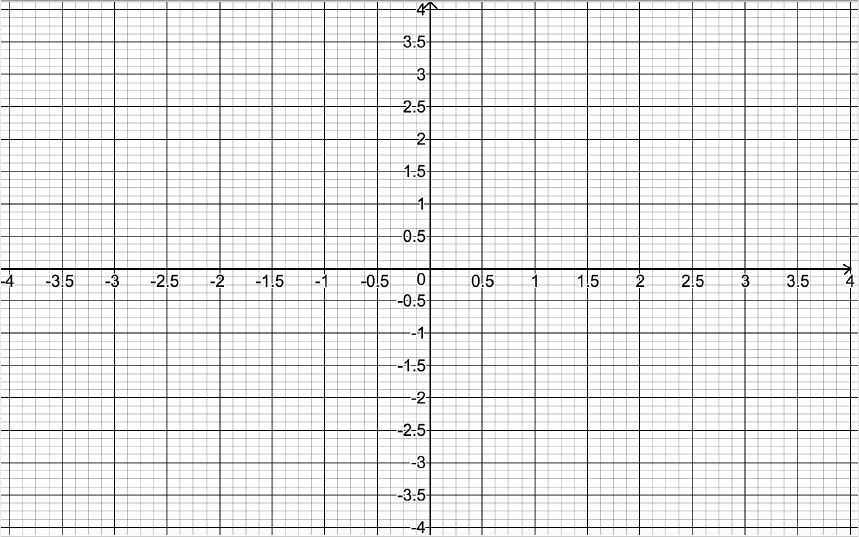
\includegraphics [scale=0.7]{Axis-Ex3.png} %%This is on CoCalc
\end{problem}



%%Problem 11%%
\begin{problem}
You are to build a box with a \textbf{square base and no top}. 

The box must hold a volume of 100 cm$^3$. 

A picture of the box is provided below. You must add labels (i.e. variables in place of $a$, $b$ and $c$) for the dimensions of the box. You will use these labels throughout the problem.
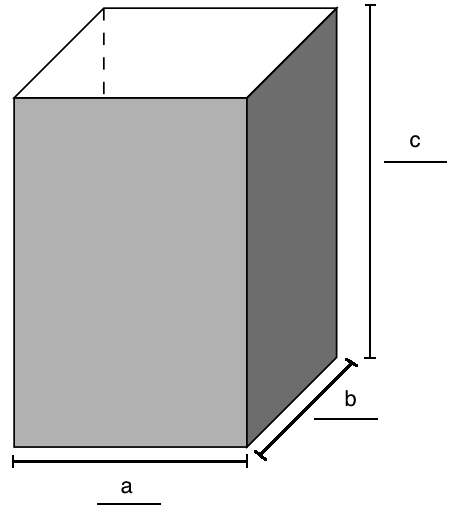
\includegraphics[scale=0.25]{Boxlabels.png} 

\begin{question}
Label each side of the box with a variable (i.e. $x$, $y$, etc.). Remember that the box has a square base.
    \[
	\displaystyle  a =    \answer[given]{x}
	\]
    \[
	\displaystyle  b =    \answer[given]{x}
	\]
    \[
	\displaystyle  c =    \answer[given]{y}
	\]
\end{question}

\begin{question}
Complete the equation for the volume of the box using the labels provided in your picture:
	\[
	\displaystyle  100 =    \answer[given]{x^{2}y}
	\] 
\end{question}

\begin{question}
Complete the equation for the surface area of the box using the labels you provided: 
    \[
	 \displaystyle Surface \, Area =  \answer[given]{x^{2}+4xy}
    \]
\end{question}

\begin{question}
Using calculus, find the dimensions of the box that require the least material for the five sides. Support your work by using \textbf{second derivative test}. 
	\[
	\displaystyle  x = \answer[given]{400^{1/3}} 
	\]
	\[
	\displaystyle y = \answer[given]{\frac{100}{400^{2/3}}}
	\]
\end{question}

\begin{question}
\underline{Justification}: Provide a 1-2 sentence explanation justifying why your solution is the optimal solution (i.e. why it is the absolute minimum). Be sure to discuss the domain and endpoints. \\(Note that this question cannot be validated in this system.)
\begin{freeResponse}
\end{freeResponse}
\end{question}

\end{problem}


%%Problem 12%%
\begin{problem}
Indicate whether each of the following statements is \textbf{True} or \textbf{False}.
 
If the statement is true, explain how you know it's true.\\
 
If it is false, give a counterexample \textbf{and} explain why it is a counterexample. (A counterexample is an example of a function for which the ``if'' part of the statement is true, but the ``then'' part is false.) \underline{A graph with an explanation can be used as a counterexample.}\\

\begin{question}
The function $f$ is continuous and positive on $[-1,1]$. If $\displaystyle\int_{-1}^1 f(x) \, dx$ is approximated with $n=4$ rectangles of equal size, then right endpoints will provide an estimate that is larger than the estimate provided using left endpoints. 
\begin{multipleChoice}
	\choice {True.}
	\choice [correct]{False.}
\end{multipleChoice}
\end{question}

\begin{question}
If a function, $g$, is continuous and increasing on $[0,3]$, then $\displaystyle\int_0^3 g(x)\,dx>0$.
\begin{multipleChoice}
	\choice {True.}
	\choice [correct]{False.}
\end{multipleChoice}
\end{question}

\end{problem}


%%Problem 13%%
\begin{problem}
Evaluate the following integrals.

\begin{question}
$\displaystyle\int\left(\frac{1}{x^2}+\sec^2(x)+2\pi\right)dx$
	\[
	\displaystyle  =    \answer[given]{-\frac{1}{x}+\tan{x}+2x\pi}+C
	\]
\end{question}

\begin{question}
$\displaystyle\int\left(t\cdot\sqrt[3]{t}\right)dt$
	\[
	\displaystyle  =    \answer[given]{\frac{3t^{7/3}}{7}}+C
	\]
\end{question}

\begin{question}
$\displaystyle\int_{0}^3\sqrt{9-x^2}\,dx$
	\[
	\displaystyle  =    \answer[given]{\frac{9\pi}{4}}
	\]
\end{question}

\end{problem}
















\end{document}